\chapter{系统需求分析}
\vspace{7pt}

在明确自动化用例建模系统的技术基础之后，本章进一步从工程实践角度对系统的功能与性能需求展开分析。首先提出系统的总体目标，界定目标用户群体并梳理核心业务流程；随后从项目管理、文档解析、智能拆解、多类型图表生成及人机交互确认等方面详细阐述功能需求，并基于需求分析结果构建系统用例模型；最后对响应时延等非功能性需求进行说明，为后续系统设计与实现提供明确的约束依据。

\section{系统总体目标}

自动化用例建模系统的总体目标是构建一个智能化的UML建模辅助平台，以自然语言需求文档为输入，利用大语言模型的语义理解能力自动完成用例图、类图与时序图的生成工作，并通过人机协作机制确保建模结果的准确性与可用性。系统旨在显著降低传统手工建模的人力成本和时间消耗，消除因分析人员认知差异导致的建模不一致问题，为软件工程实践中的需求分析与设计阶段提供高效可靠的技术支撑。

具体而言，系统的目标可以分解为三个层面。在功能层面，系统需要覆盖从需求文档导入、智能模块拆解、多类型图表自动生成到建模成果导出的完整链路。用户仅需上传需求文档并进行少量确认操作，即可获得符合UML规范的用例图、类图和时序图。在质量层面，系统需要保证生成图表中实体识别的完整性与关系推理的正确性，同时确保输出的PlantUML代码具有百分之百的语法合法性，能够被渲染引擎直接渲染为图片。在体验层面，系统需要提供直观易用的可视化界面，支持用户在自动生成的基础上进行人工修正和微调，实现人机协同的增量式建模过程。

\section{用户角色与业务流程分析}

\subsection{业务流程总体分析}

本系统的目标用户群体主要包括三类角色。第一类是系统分析师，他们负责阅读和分析需求文档，识别系统功能边界并构建用例模型。系统分析师是系统的核心用户，他们将使用系统完成大部分建模操作。第二类是软件架构师，他们在接收到用例模型后进行高层设计，需要查看、验证和可能修改用例图与类图，确保模型与设计意图一致。第三类是项目管理人员，他们可能仅需要查看生成的UML图表，以了解系统功能范围，用于项目进度评估和沟通协调。

系统的核心业务流程围绕需求文档的输入、处理和输出展开。用户首先创建项目并上传需求文档，系统提供文本文件和PDF文件两种输入渠道。对于复杂项目，用户可以选择启用智能模块拆解功能，由系统自动识别文档中的功能模块划分。在建模阶段，用户选择目标图表类型，系统启动多智能体工作流，依次提取建模要素并在关键节点暂停等待用户确认。用户可以在表格界面中查看、修改和确认提取结果，确认后的数据将被锁定，防止后续处理中发生意外变更。确认完成后，系统基于最终数据生成PlantUML代码并渲染为可视化图形。用户还可以在Monaco编辑器中对代码进行微调，调整后的代码将与数据表格保持双向同步。用户确认满意后可将生成的UML模型与代码一并导出。

系统的总体业务流程如图3.1所示。

% 图3.1 建模系统总体业务流程图
\begin{figure}[htbp]
    \centering
    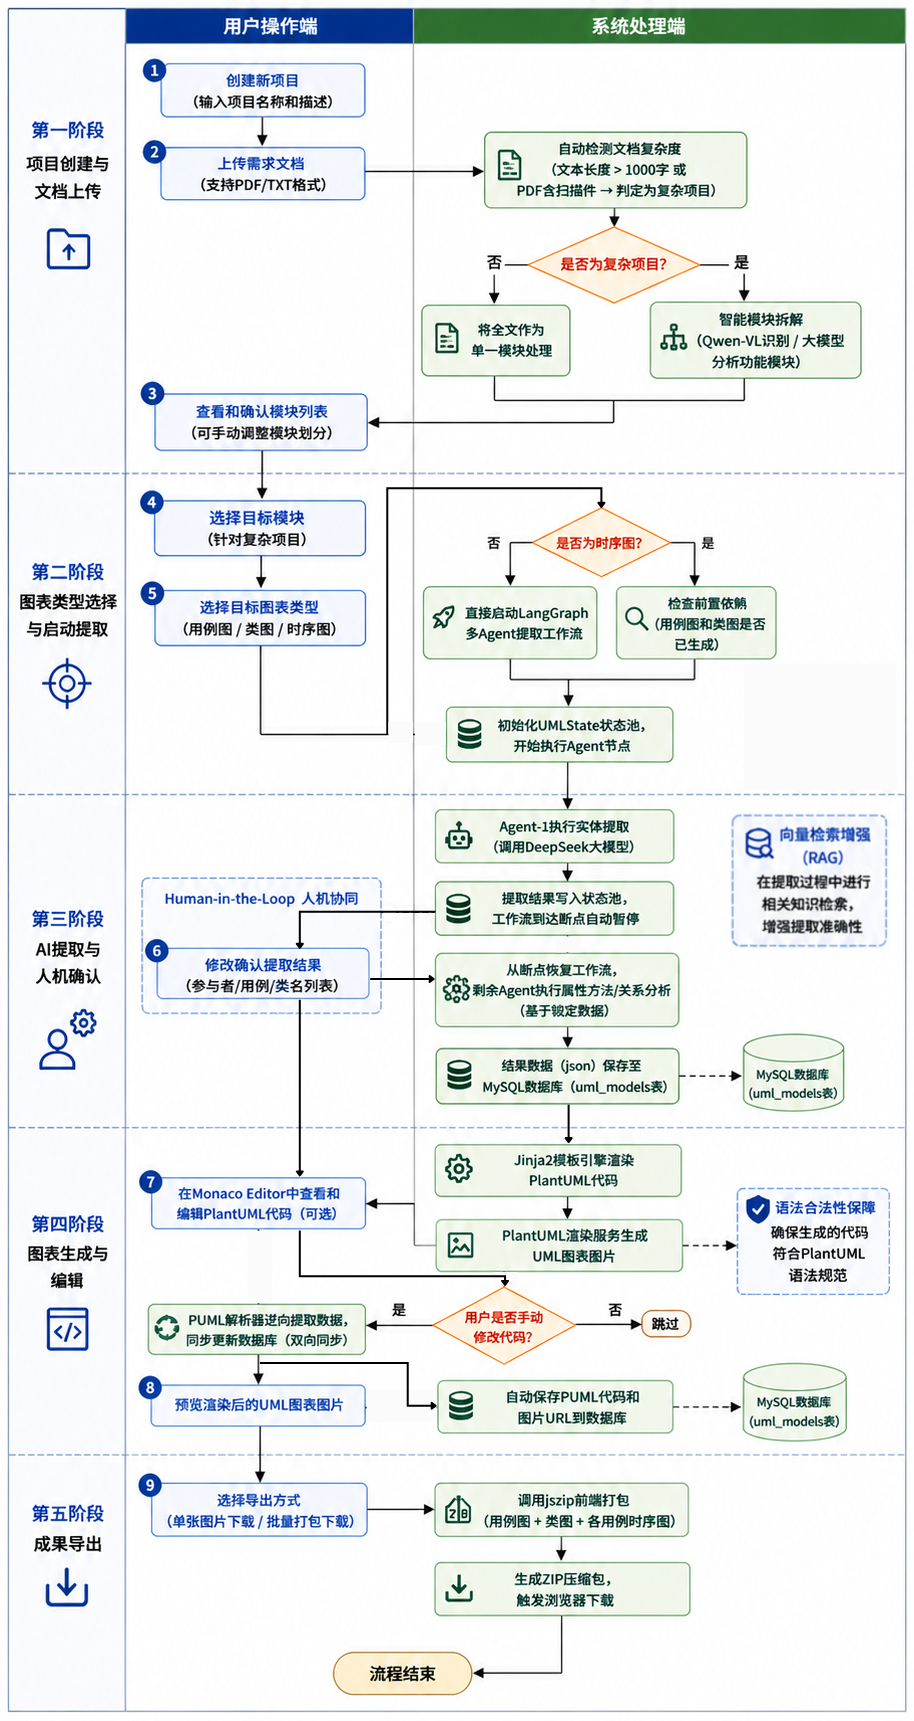
\includegraphics[width=120mm]{docs/imgs/建模系统总体业务流程图.png}
    % \vspace{-8pt}
    % \fontSimsun\sizeFive 图3.1 建模系统总体业务流程图
    % \vspace{-8pt}
    \caption{建模系统总体业务流程图}
    \label{fig:business_flow}
\end{figure}

\section{功能需求分析}

\subsection{项目管理与多模态文档解析需求}

系统需要提供完善的项目全生命周期管理功能。用户应当能够创建新项目，为项目指定名称和描述信息。对于需要分模块处理的复杂项目，系统应当支持在项目下划分子模块，每个模块对应需求文档中的一个功能区域。项目数据需要持久化存储，用户可以在任意时刻恢复之前的工作进度，继续未完成的建模任务。

多模态文档解析是系统的入口功能，直接决定了后续提取质量的基础。系统需要支持两种类型的文档输入。对于纯文本格式的需求文档，系统应当能够直接读取文件内容并交由后续处理流程。对于PDF格式的文档，系统需要区分文本型PDF和扫描型PDF两种情况。文本型PDF通过PDF文本提取库直接抽取文字内容，保留原有的段落结构和文本顺序。扫描型PDF则需要调用多模态视觉模型对页面图片进行光学字符识别，将识别结果重新组织为文本。系统还需要支持上传PDF文件时的中英文混合内容处理，确保在含有多语言术语的需求文档中不会出现字符乱码或内容丢失。

\subsection{复杂项目智能模块拆解需求}

在实际工程场景中，一份完整的需求规格说明书往往涵盖系统的多个功能子系统。例如，一个企业资源计划系统的需求文档可能同时包含采购管理、库存管理、生产管理和财务管理等多个模块的内容。如果直接对整份文档进行用例提取，不仅会因为文本篇幅过长导致模型的信息丢失，还会生成一张过于庞杂而难以阅读的用例图。因此，系统需要提供智能模块拆解功能。

该功能需要由大语言模型对上传的需求文档进行结构性分析，识别文档中描述的不同功能模块，并为每个模块提取核心需求描述。拆解结果以模块列表的形式呈现给用户，用户可以对模块名称和范围进行确认和调整。每个模块将拥有独立的建模空间，用户可以在不同模块之间切换，分别进行用例图、类图和时序图的生成。模块拆解的粒度需要适中，既要避免粒度过细导致模块间关系难以体现，也要避免粒度过粗失去分模块建模的意义。

\subsection{用例图、类图、时序图自动化生成需求}

三类UML图表的自动化生成是系统的核心功能需求。对于用例图，系统需要从需求文本中提取系统参与者和用例名称，并分析它们之间的包含关系、扩展关系和泛化关系。提取的参与者应当涵盖人类用户、外部系统和时间触发器等不同类型。用例的提取应当聚焦于具有独立业务价值的系统功能，而非颗粒度过细的操作步骤。关系分析需要结合需求文本中的条件描述和前置依赖信息进行综合判断。

对于类图，系统需要完成三个层次的提取工作。第一层是实体类的识别，从需求文档中找出代表核心业务概念的类名。第二层是类属性与方法的提取，需要从文本描述中分析每个实体类应包含的关键属性和操作。第三层是类间关系的推理，包括关联、聚合、组合、继承和接口实现等多种关系类型的判定。类图的生成需要保证属性和方法与类的归属关系正确，类间关系的多重性标注合理。

对于时序图，系统需要针对每个用例分析其参与者构成和消息交互序列。参与者的提取需要明确列出参与交互的角色或外部系统。消息序列的编排需遵循业务逻辑的时间顺序，准确反映参与者之间的消息传递方向和调用层次，从而完整描述用例执行过程中的动态行为。

\subsection{人机交互确认与双向代码编辑需求}

自动化生成的结果不可避免地存在边界情况上的误差，系统需要提供灵活的人机交互机制使用户能够对中间结果进行审查和修正。在用例图生成流程中，实体提取完成后、关系分析开始前设置确认断点供用户修正；类图生成则在类名提取完成后设置确认断点，后续提取基于确定类名进行，避免模型自行新增类名。这种半自动化的交互设计在近期的前沿研究中被证明是必不可少的。Eisenreich等人\cite{eisenreich2025leveraging}在进行大语言模型建模的实证研究中指出，完全自动化的生成流程常常导致模型更高概率产生幻觉，因此强烈建议采用半自动化的工作流。通过让用户在每个关键提取步骤后进行验证和干预，不仅能修正模型的误解，还能显著增强用户对建模结果的控制感与信任度。

数据表格与PlantUML代码编辑器之间的双向同步是另一项重要的交互需求。当用户在前端表格中修改实体名称或关系数据时，系统需要即时重新渲染PlantUML代码并更新编辑器显示。反之，当用户在编辑器中直接修改PlantUML代码的合法部分时，系统需要解析代码中的实体和关系声明，反向更新数据表格的内容。这一同步机制使用户可以在图形化操作和文本编辑两种模式之间自由切换，系统需要保证同步过程的实时性以及两个视图数据的一致性。

\section{系统用例建模}

基于上述功能需求分析，本文对本自动化用例建模系统自身进行了用例建模。系统的主要用例包括项目管理、需求文档上传与解析、智能模块拆解、用例图生成、类图生成、时序图生成、提取结果确认与修改、PlantUML代码编辑与同步、以及建模成果导出。用例之间的关联关系体现了系统的流程约束：所有 UML 图表生成用例均包含查看确认提取结果用例，这一设计将人工校验作为生成流程的强制环节，可有效降低自动化抽取过程中的信息偏差；智能模块拆解用例作为扩展用例，扩展了上传需求文档的基础流程，当用户上传的文档被判定为复杂项目时，可选择启动模块拆解以提升后续建模的完整性与准确性。系统的总体用例模型如图 3.2 所示。

系统的总体用例图如图3.2所示。
% 图3.2 系统总体用例图
\begin{figure}[htbp]
    \centering
    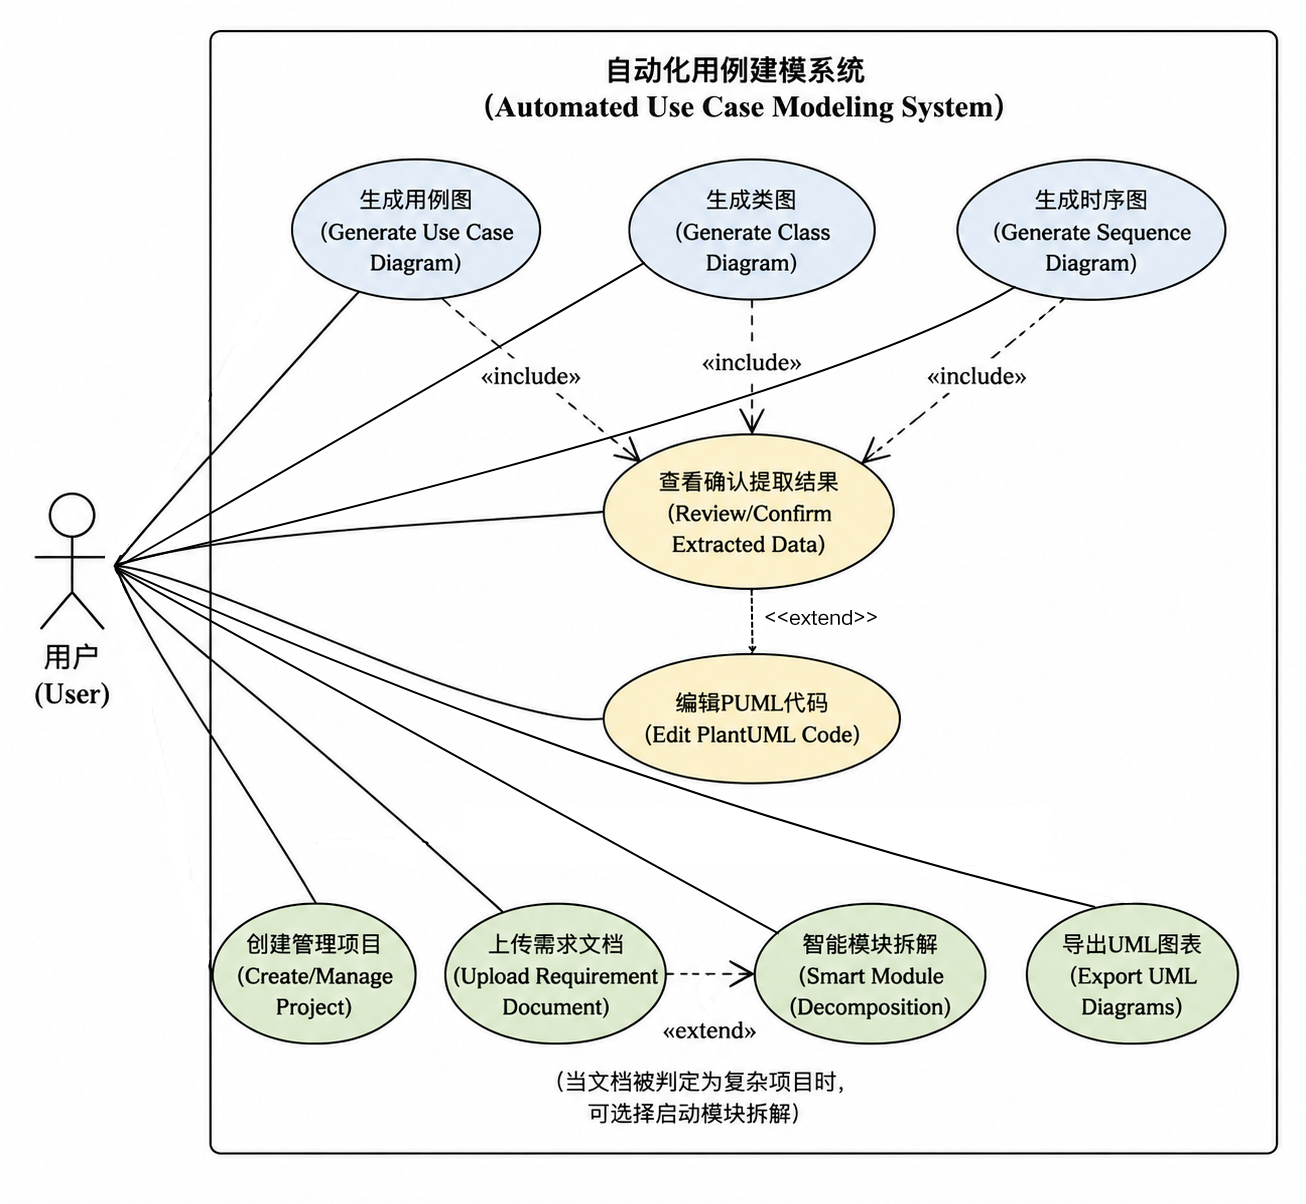
\includegraphics[width=100mm,height=100mm]{docs/imgs/系统用例图.png}
    % \vspace{-8pt}
    % \fontSimsun\sizeFive 图3.2 系统总体用例图
    % \vspace{-8pt}
    \caption{系统总体用例图}
    \label{fig:system_usecase}
\end{figure}

\section{系统非功能性需求}

\subsection{模型推理响应时延}

系统的用户体验在很大程度上取决于智能分析环节的响应速度。当用户提交需求文本进行用例提取或关系分析时，系统需要调用外部大语言模型服务完成推理计算。考虑到用户在工作流中的等待容忍度，单次推理请求的响应时延应控制在可接受的时间范围内。对于常规篇幅的模块需求文本，实体提取节点的响应时延不应超过十五秒。对于关系分析和类属性方法提取等需要处理更复杂语义的任务，响应时延可以适当放宽，但不应超过六十秒。

系统的整体时延表现受到多个因素的影响，包括输入文本的长度、模型服务的并发负载以及网络通信延迟。因此，在系统设计中需要考虑多方面的优化策略，例如通过RAG检索控制输入提示词的长度，合理设置模型服务的请求超时与重试机制，以及在前端通过加载状态提示和进度动画来改善用户的主观等待体验。

\section{本章小结}

本章围绕自动化用例建模系统的需求展开系统分析，明确了系统的总体目标与三类用户角色，绘制了核心业务流程图。在功能需求方面，涵盖了多模态文档解析、智能模块拆解、用例图/类图/时序图自动生成以及人机交互确认与双向代码编辑等关键需求，并据此构建了系统用例模型。在非功能需求方面，重点提出了模型推理响应时延的指标要求。上述分析为第四章的系统设计奠定了完整的需求基础。